\documentclass{article}
\usepackage{tikz, comment}
\usepackage{pifont}
\usepackage{fontspec}
\usetikzlibrary{arrows, decorations.markings, decorations.pathreplacing}
\begin{comment}
:Title: Not defined yet
:Tags: 
:Author: Prof.Hu Ji-shan, HKUST
:Slug: No name yet

Description Here.........
\end{comment}
\begin{document}\centering

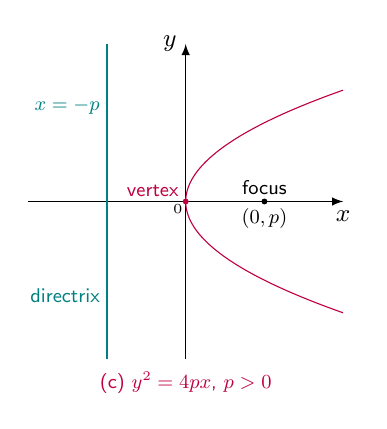
\begin{tikzpicture}[>=latex,xscale=.5*1, yscale=.5*1][font=\sf\small]

\draw[->] (-4, 0) -- (4, 0)node[below] {\small $x$};
\draw[->] (0, -4) -- (0, 4)node[left] {\small $y$};

\node[purple, scale=0.8] at (0, -4.6) {(c) $y^2 = 4px$, $p > 0$};

\clip[] (-4,-4) rectangle (4,4);

\draw[purple, samples=100, smooth, domain=-3:3, variable=\y]
plot ({1/4*2*(\y)^2}, {\y}) ;

\draw[teal] (-2,-4) -- (-2, 4) node[left, pos=0.2, scale=0.8]{$\hbox{directrix}$} node[left, pos=0.8, scale=0.8]{$x=-p$};

\draw[fill] (2, 0) circle(0.06) node[above, scale=0.8]{$\hbox{focus}$} node[below, scale=0.8]{$(0, p)$};

\draw[purple, fill] (0, 0) circle(0.06)node[left, yshift= 4, scale=0.8]{$\hbox{vertex}$};

\node at (-0.2/1, -0.2/1) {\tiny$0$};

\end{tikzpicture}\hskip1cm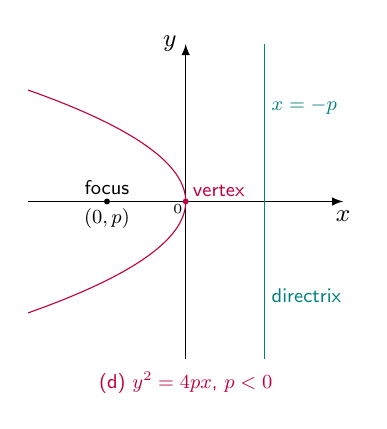
\begin{tikzpicture}[>=latex,xscale=.5*1, yscale=.5*1][font=\sf\small]

\draw[->] (-4, 0) -- (4, 0)node[below] {\small $x$};
\draw[->] (0, -4) -- (0, 4)node[left] {\small $y$};

\node[purple, scale=0.8] at (0, -4.6) {(d) $y^2 = 4px$, $p < 0$};

\clip[] (-4,-4) rectangle (4,4);

\draw[purple, samples=100, smooth, domain=-3:3, variable=\y]
plot ({-1/4*2*(\y)^2}, {\y}) ;

\draw[teal] ( 2,-4) -- ( 2, 4) node[right, pos=0.2, scale=0.8]{$\hbox{directrix}$} node[right, pos=0.8, scale=0.8]{$x=-p$};

\draw[fill] (-2, 0) circle(0.06) node[above, scale=0.8]{$\hbox{focus}$} node[below, scale=0.8]{$(0, p)$};

\draw[purple, fill] (0, 0) circle(0.06)node[right, yshift= 4, scale=0.8]{$\hbox{vertex}$};

\node at (-0.2/1, -0.2/1) {\tiny$0$};

\end{tikzpicture}
\end{document}